\documentclass[fleqn]{article}
\usepackage[UTF8]{ctex}
\usepackage{listings}
\usepackage{pdfpages}
\usepackage{color}
\usepackage[colorlinks,linkcolor=blue]{hyperref}
\usepackage{dashrule}
\usepackage{diagbox}
\usepackage[german]{babel}
\usepackage[T1]{fontenc}
\usepackage[latin1]{inputenc}
\usepackage{titlesec}
\usepackage{geometry}
\usepackage{qtree}
\usepackage{tikz}
\usepackage{amsmath}
\usepackage{amssymb}
\setcounter{secnumdepth}{0}
\usetikzlibrary{positioning}
\geometry{top=2.5cm, bottom=2.5cm}
\lstset{
 columns=fixed,       
 numbers=left,                                        % 在左侧显示行号
 numberstyle=\tiny\color{gray},                       % 设定行号格式
 frame=none,                                          % 不显示背景边框
 backgroundcolor=\color[RGB]{245,245,244},            % 设定背景颜色
 keywordstyle=\color[RGB]{40,40,255},                 % 设定关键字颜色
 numberstyle=\footnotesize\color{darkgray},           
 commentstyle=\it\color[RGB]{0,96,96},                % 设置代码注释的格式
 stringstyle=\rmfamily\slshape\color[RGB]{128,0,0},   % 设置字符串格式
 showstringspaces=false,                              % 不显示字符串中的空格
 language=c++,                                        % 设置语言
 breaklines,                                          % 自动换行
}

\title{RO Zusammenfassung WS20/21}

% \author{Dongze Yang}

\begin{document}

\maketitle

\newpage

\textit{Stand der Zusammenfassung:} WS 2020/2021

\textit{Genutzte Quellen:} 

\indent\indent Portfolio und Zusammenfassung ,,Rechnerorganisation'' WS 2017/18

\indent\indent Vorlesungs- Übungsfolien zur Verfügung gestellt über OPAL

\textit{Zuletzt gesichtet am 10.02.2021 9:00 Uhr} 

\newpage

\tableofcontents

\newpagestyle{main}{
    \sethead{}{}{RO WS20/21}
    \setfoot{}{\thepage}{}
    \headrule
    \footrule
}
\pagestyle{main}

\newpage

\section{Gesetz von Amdahl}

Die Verbesserung der Gesamtleistung durch die Verbesserung einer Systemkomponente ist auf denZeitanteil begrenzt, in dem die verbesserte Komponente genutzt wird.

通过改进系统组件来提高总体性能,仅限于使用改进的组件的时间比例。

\noindent \underline{Bsp.}

\noindent \textit{Gegeben ist ein sequentielles Programm aus 3 Teilen.}

\textit{A: 3 Zeiteinheiten}

\textit{B: 2 Zeiteinheiten}

\textit{C: 5 Zeiteinheiten}

\noindent \textit{Optimierungsmöglichkeiten:}

\textit{A : 5 mal so schnell}

\textit{B : 10 mal so schnell}

\textit{C : 2 mal so schnell}

\noindent\textit{Welche Optimierungsmöglichkeit bringt den größten Vorteil?}
\\
\\
\textbf{Ans:C}. Für A: 2.4 ZE ($3\times(1-\frac{1}{5})$), für B ZE ($2\times-\frac{1}{10}$), für C ZE ($5\times(1-\frac{1}{2})$)

\begin{center}
    \begin{tabular}{|c|c|c|c|c|}
        \hline
        &A&B&C&Summe\\
        \hline
        Zeiteinheiten T &3&2&5&10\\
        \hline
        Optimierung S&5&10&2&\\
        \hline
        Anteil P&0.3&0.2&0.5&1\\
        \hline
        \hline
        in \%&24&18&25&\\
        \hline
        Resultierende Zeit&10-2.4=7.6&8.2&7.5&\\
        \hline
        \hline
        Speedup S&10/7.6=1.31578947&1.2195122&1.33333333&\\
        \hline
    \end{tabular}
\end{center}
\section{Gesetz von Moore}

Das Gesetz von Moore sagt den Fortschritt bei der Integration von Transistoren voraus. 
摩尔定律预测了晶体管集成的进展。

$\rightarrow$ Die Anzahl der Transistoren in einem Chip verdoppelt sich alle 18 Monate. 芯片中的晶体管数量每18个月翻一番。

Problem: Bald erreicht man physikalische Grenzen. 问题:很快就达到了物理极限。

\section{Harvard-Architektur und Neumann-Architektur}

\begin{center}
    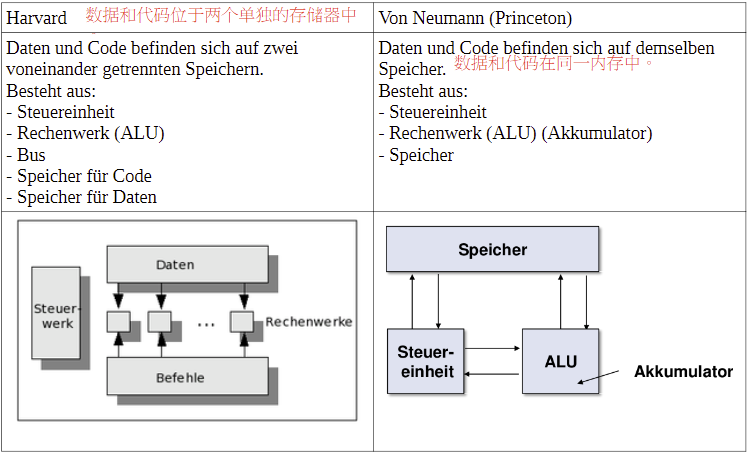
\includegraphics[scale=0.5]{1.png}
\end{center}

\section{RISC und CISC}

\begin{center}
    \begin{tabular}{|l|l|}
        \hline
        RISC 精简- & CISC 复杂指令集计算机\\
        \hline
        Reduced Instruction Set Computer & Complex Instruction Set Computer\\
        - Beschränkung auf einen einfachen Befehlssatz & - erweiterter Befehlssatz\\
        - schnelle Abarbeitung & - langsamer in der Ausführung\\
        \hline
    \end{tabular}
\end{center}

\section{Big-Endian und Little-Endian}

Bei Big-Endian wird das höherwertige Byte zuerst gespeichert, das heißt an der kleinsten Speicheradresse.

使用大端序时,最高有效字节先保存,即保存在最小的内存地址中。

Bei Little-Endian wird dagegen das kleinstwertige Byte an der Anfangsadresse gespeichert.

但对于小端序,最低有效字节存储在起始地址中。

\section{Hamming}

Der Hamming-Algorithmus dient im Allgemeinen dazu, Fehler in Bit-Wörtern zu finden und ggf. zu korrigieren.

汉明算法通常用语查找位字中的错误,并在必要时纠正。

\noindent Hammingabstand = Anzahl verschiedener Bits zweier Wörter.

$\rightarrow$ Um $d$ Einzelbitfeler zu erkennen (确认d个错误), benötigt man einen Code mit einem Abstand von $d+1$

$\rightarrow$ Um $d$ Einzelbitfehler zu korrigieren (改正d个错误), benötigt man einen Code mit einem Abstand von $2d+1$
\\
\\
In Datenspeicherung: ist die kleinste Anzahl der Prüfbits, um Einzelbitfehler zu korrigieren
在数据存储中:是纠正单个位错误的最小校验位数:

$(n+1)\cdot 2^m \leq 2^n \rightarrow (m+r+1)\leq 2^r$

\noindent(Code mit $m$ Datenbits und $r$ Prüfbits, $n$-Bit-Codewort $n=m+r$, Gesamtzahl der Bitmuster $2^n$)

\subsection{Vorgehensweise Hamming-Algorithmus:}

1) Bitwort besteht aus den Stellen 1 bis n. An jeder $2^n$-ten Stelle setzen wir ein Paritätsbit.
位字由位置1到n组成,我们在每个$ 2 ^ n $-ten位置设置一个奇偶校验位。

2) Das Paritätsbit an der Stelle $n$ zu finden, springt man von da aus $n$ Stellen und betrachtet die Nachfolgenden $n$ Stellen, springt wieder $n$ Stellen,$\dots$ bis das Wort zu Ende.
要在$ n $位置找到奇偶校验位,请从那里跳转到$ n $位置并查看以下$ n $位置,然后跳转到$ n $位置,$ \cdots$直到单词结束。

3) Man betrachtet die Anzahl der Einsen und Nullen in den DATENBITS: Gerade $\#1 = 0$, Ungerade $\#1 = 1$
考虑数据位中的1和0的数目:偶$ \#1 = 0 $,奇数$ \#1 = 1 $

4) Die Position eines falschen Bits lässt sich finden, indem man die Position aller falschen Paritätsbit addiert.
可以通过添加所有错误的奇偶校验位的位置来找到错误的位的位置。
\\
\\
\underline{Ein Fehlerkorrekturcode erfordert eine Anzahl an Prüfbits, die immer doppelt so viel wie die}

\underline{Anzahl der Datenbits ist.} (Falsch)

\underline{纠错码需要一定数量的校验位,该校验位总是数据位数的两倍。} (错)

\subsection{möglichen Fragen:}

\textbf{1.} Was repräsentiert der Hammingabstandzwischen zwei Codewörtern? Berechnen sie diesen für 1001 0010 und 1000 0011. Welche Paritätsbits haben diese beiden Codewörter? Wievielezusätzliche Korrekturbits sind für Codewörter der Länge 8 notwendig?

两个代码字之间的汉明距离代表什么? 为1001 0010和1000 0011计算此值。这两个代码字具有哪些奇偶校验位? 长度为8的代码字需要多少个其他校正位?

a) Anzahl sich unterscheidender Bitstellen. Hier im Beispiel: 2

b) Paritätsbits sind beide 1 (ungerade Anzahl 1-Bits)

c) $(m+r+1)\leq 2^r$, wobei m = Länge und r = Anzahl Prüfbits $\rightarrow$ 4 Prüfbits
\\
\\
\noindent\textbf{2.} Wie werden Fehlerkorrekturbits zur Erkennung von Einzelbitfehlern genutzt? Beschreiben sie eine Möglichkeit für das Codewort1010 (3 Prüfbits).

纠错位如何用于检测单个位错误? 描述代码字1010(3个校验位)的可能性。

Bits B1 bis B4, Prüfbits A B C $\rightarrow$ Wort B1 B2 B3 B4 A B C

A = B1 + B2 + B4, B = B1 + B2 + B3, C = B1 + B3 + B4

B1 = A + B + C, B2 = A + B, B3 = B + C, B4 = A + C 

\begin{center}
    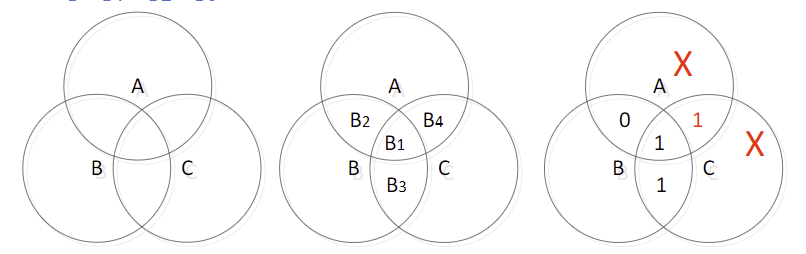
\includegraphics[scale=0.5]{7.png}
\end{center}

\noindent\textbf{3.} Welche Paritätsbits haben die nachfolgenden Codewörter bei der Fehlerkorrektur nach dem Hamming-Algorithmus?
a) 10\underline{1}0, b) 1011 1\underline{0}10. Woran erkennen Sie einen Bitfehler an den farbig markierten Bits?

以下代码字具有哪些奇偶校验位以根据汉明算法进行纠错?
a)10\underline{1}0,b)1011 1\underline{0}10。 您如何识别彩色位上的位错误?

\noindent Hinweis:
\begin{center}
    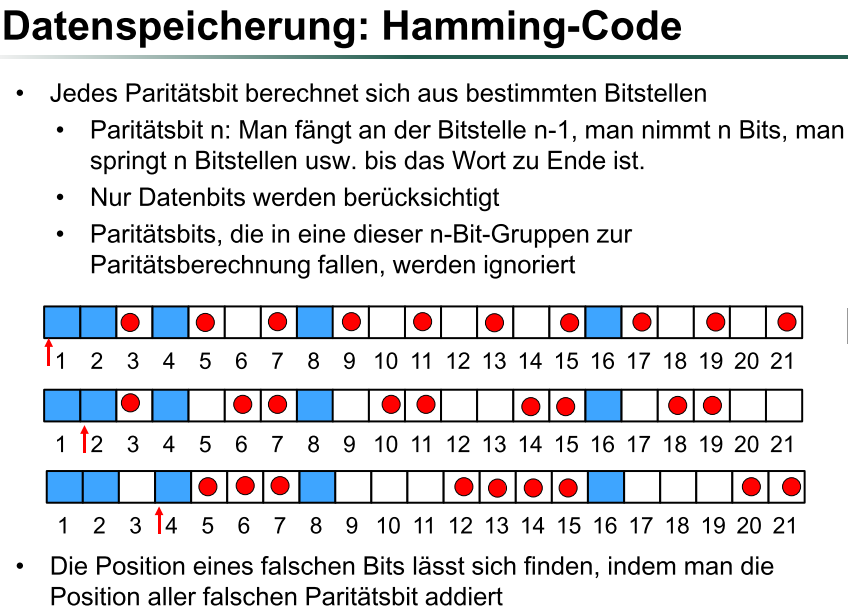
\includegraphics[scale=0.5]{8.png}
\end{center}

\textbf{Lösung:}

Paritätsbits:

a) 101

b) 0000

Bitfehler:

a) PB2 und 4

b) PB2 und 8

Summe der Stellen der

Paritätsbits = Fehlerstelle
\\
\\
\noindent\textbf{4.} Mit dem Hamming-Algorithmus können lediglich Einzelbitfehler erkannt werden.(Falsch)

使用汉明算法,只能检测到单个位错误。(错)

\section{Logikschaltungen}

\subsection{4-Input-Multiplexer} 复用器

Schaltung mit $2^n$ Dateneingängen, einem Datenausgang und n Steuereingängen, die einen der Dateneingängen auswählen.

具有$2^n$个数据输入,一个数据输出和$n$个控制输入的电路。用于选择数据输入之一。

\begin{center}
    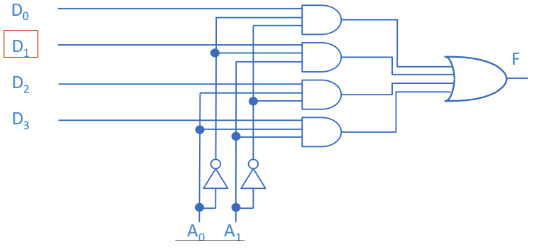
\includegraphics[scale=0.6]{2.png}
\end{center}

\subsection{Decodierer} 解码器

Schaltung, die eine n-Bit-Zahl als Eingabe übernimmt und dieser Zahl entsprechend genau eine der $2^n$ Ausgangsleitungen wählt.

接受$n$位数字作为输入,并根据该数字选择$2^n$条输出线之一的电路。

\subsection{4-Bit-Komparator} 比较器

Schaltung, die zwei Eingangswörter vergleicht. 比较两个输入字的电路。

\begin{center}
    \begin{tabular}{|c|c|c|}
        \hline
        A&B&Y\\
        \hline
        0&0&0\\
        0&1&1\\
        1&0&1\\
        1&1&0\\
        \hline
    \end{tabular}
\end{center}

\begin{center}
    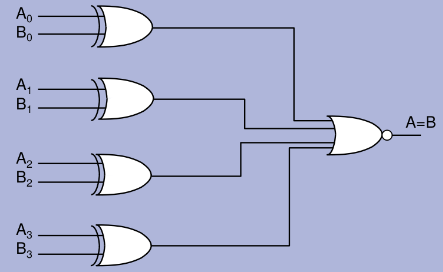
\includegraphics[scale=0.6]{3.png}
\end{center}

\subsection{Halbaddierer} 半加器

Schaltung, die Summen- und Übertrags-Bit berechnet, ohne den einlaufenden Übertrag zu berücksichtigen.

在不考虑传入进位的情况下,计算总和和进位的电路。

\begin{center}
    \begin{tabular}{|c|c|c|c|}
        \hline
        A&B&S&Ueb\\
        \hline
        0&0&0&0\\
        0&1&1&0\\
        1&0&1&0\\
        1&1&0&1\\
        \hline
    \end{tabular}
\end{center}
\begin{center}
    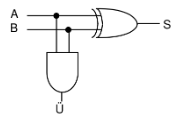
\includegraphics[scale=0.6]{4.png}
\end{center}

\subsection{Volladdierer} 全加器

Wie Halbaddierer, nur unter Berücksichtigung des Übertrages.

\begin{center}
    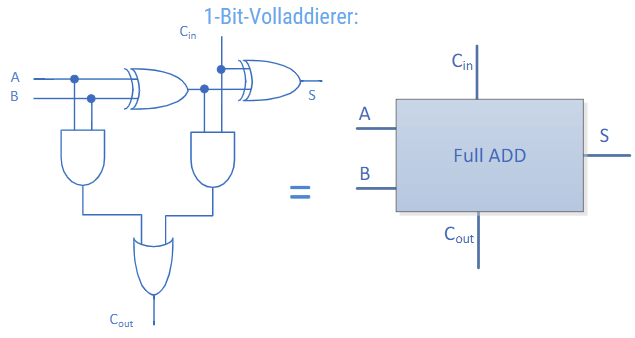
\includegraphics[scale=0.6]{5.png}
    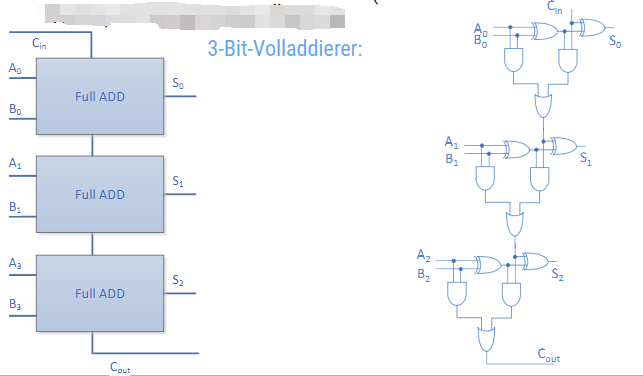
\includegraphics[scale=0.6]{10.png}
\end{center}

\section{Flankendifferenzierer}

边缘微分器。

Der Impuls eines Taktes kann verhältnismäßig lang sein und verursacht dadurch Instabilität. Durch den Flankendifferenzierer soll diese eingefangen werden.

Taktes的脉冲可能相对较长,因此会导致不稳定。这应该由边缘微分器捕获。

\noindent\underline{Bsp.}

Angenommen, ein Negationsgatter hat ein Delay von 40ns - Wie viele Negationsgatter sind nötig, um eine Flanke mit einem $\Delta$ = 240ns Signal zu differenzieren?

假设求反门具有40ns的延迟 - 需要多少个求反门来区分$\Delta$ = 240ns信号的边沿?

\begin{center}
    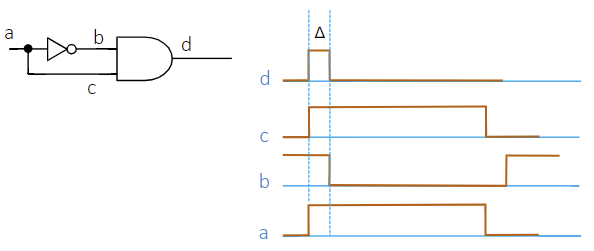
\includegraphics[scale=0.6]{11.png}
\end{center}

$240/40=6$, aber eine gerade Anzahl an Differenzieren ändert am Eingangssignal nichts, deshalb +1.

$\rightarrow$ Es werden 7 Gatter benötigt.

\subsection{Latches und Flip-Flops}

Ein Latch ist ein Schaltwerk mit innerem Zustand und bildet daher eine Speicherzelle. Sie können auch synchron mit dem Takt eingelesen werden.

锁存器是具有内部状态的开关机构,因此可构成存储单元。他们也可以与始终同步读取。

\begin{center}
    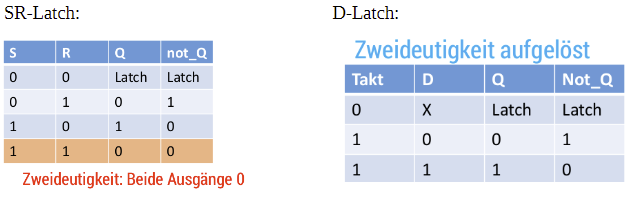
\includegraphics[scale=0.6]{6.png}
    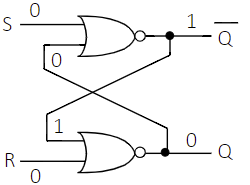
\includegraphics[scale=0.6]{12.png}
    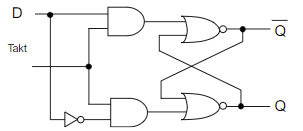
\includegraphics[scale=0.6]{13.png}
\end{center}

\noindent\underline{Nutzen/Anwendungsbereich eines D-FF}

\begin{center}
    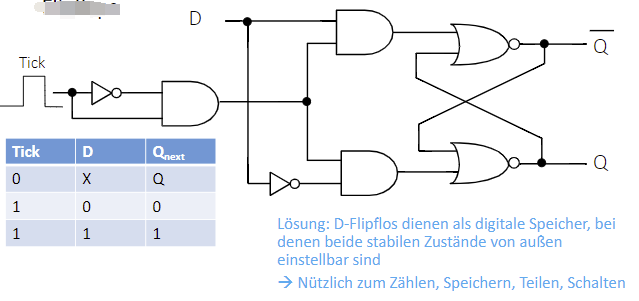
\includegraphics[scale=0.6]{14.png}
\end{center}

\noindent\underline{Der Unterschied zwischen einem D-Flipflop und einem D-Latch besteht nur darin, dass der D-}

\underline{Flipflop flankengesteuert ist.} (Richtig)

\underline{D触发器和D闩锁之间的唯一区别是D触发器是边沿触发的。} (对)

\section{Caches}

\noindent Cache ist ein schneller, integrierter Zwischenspeicher, der den Zugriff auf häufig verwendete Daten beschleunigt / beschleunigen soll.

\noindent 高速缓存器是一种快速的集成中间存储,可加速/加速对常用数据的访问。


\subsection{Lokalitätseigenschaft (Locality Principle):}

Computerprogramme greifen innerhalb eines gewissen Zeitabschnitts (temporale Lokalität, ein Bereich aufgerufen, wahrscheinlich bald wieder) nur auf einen kleinen Teil des gesamten Speicherraums (räumliche Lokalität, Zugriffe meist in der Nähe) zu.

在一定时间段内(时间局部性,一个被调用的区域,可能很快会再次出现),计算机程序仅访问总存储空间的一小部分(空间局部性,主要访问附近区域)。


\subsection{möglichen Fragen}

\noindent\textbf{1.} Erklären Sie Write-Through, Write-Back und Write-Allocate. 说明直写,回写和写分配

Write-Through (no-WA): Daten können sowohl auf dem Cache als auch auf dem Arbeitsspeicher geändert werden.

直写(无WA):可以在高速缓存和主存储器中更改数据。

Write-Back(WA): Daten können nur auf dem Cache geändert werden (und erst beim Verdrängen auf dem Arbeitsspeicher)

回写(WA):只能在高速缓存上更改数据(并且只有在将其移入主存储器时才可以更改)

Write-Allocate: Wenn es gibt Cache-Miss beim Schreiben, der Datenblock wird zuerst auf den Cache geladen und dann überschrieben.Cache

写入分配:如果在写入时发生高速缓存未命中,则首先将数据块加载到高速缓存中,然后再覆盖。
\\
\\
\noindent\textbf{2.} Gegeben sei ein Cache mit 64 Blöcken mit Block‐Größe 16 Bytes. Was ist die Cache‐Größe in KBits?

给出了具有16个字节块大小的64个块的高速缓存。 KBits中的缓存大小是多少?

B: Byte, b: bit. $S=64\cdot 16 = 2^6\cdot 2^4 B=2^{10}B=8\cdot 2^{10}b=8Kb$
\\
\\
\noindent\textbf{3.} Gegeben sei ein 16KB‐Cache mit 32 Byte Blockgröße. Wie verteilen sich die Bits einer 32‐Bit‐Adresse auf:

给出了具有32字节块大小的16KB高速缓存。 32位地址的位如何分配:

\begin{center}
    
\includegraphics[scale=0.5]{9.png}
\end{center}

$T_{Byte\_Offset}=32=2^5 \,(i.e.\, 4\dots0)$

$T_{Block\_Index}=\frac{16KB}{32Bytes}=\frac{16\cdot 2^10 Bytes}{32Bytes}=2^9\,(i.e.\,13\dots5)$

$T_{Tag} = \frac{2^{31}}{2^5\cdot 2^9}=2^{17}\,(i.e.\, 31\dots 14)$
\\
\\
\noindent\textbf{4.} Erklären Sie Cacheline(Block), Hit(Treffer), Miss(Verfehlen), Miss Penalty, Direct-Mapped-Cache und Set-Assoziativer Cache.

解释高速缓存行(块),命中(命中),未命中(未命中),未命中罚分,直接映射的高速缓存和集关联高速缓存。

\textbf{Cacheline(Block)}: Kleinste Datenmenge zwischen Arbeitsspeicher und Cache.

高速缓存行(块):主内存和高速缓存之间的数据量最少。

\textbf{Hit (Treffer)}: Daten sind beim Zugreifen auf dem Cache.

命中:数据在访问时在缓存中。

\textbf{Miss (Verfehlen)}: Daten sind beim Zugreifen nicht auf dem Cache.

丢失:访问数据时不在高速缓存中。

\textbf{Miss Penalty}: Zusätzliches Delay, das durch Verfehlen der Daten entsteht.Cache-Hit/Miss beim Schreiben

未命中罚款:由于丢失数据而导致的额外延迟;写入时缓存命中/未命中
\\
\\
\noindent\textbf{5.} Ein Programm hat 100.000 Befehle mit 20 Misses pro 1000 befehle, 10\% davon sind Speicherbefehle, berechnen Sie die \textbf{Missrate}.

一个程序有100,000个命令,每1000个命令有20个未命中,其中10%是存储命令,请计算\textbf {未命中率}。

$$\frac{Misses}{Befehl}=Missrate\times \frac{Speicherbefehle}{Gesamtbefehle}$$

$$Missrate = \frac{Misses}{Befehle}\div \frac{Speicherbefehle}{Gesamtbefehle}=\frac{20}{1000}\div 10\%=20\%$$

\noindent\textbf{6.}
\underline{L1, L2, L3}

Man unterscheidet L1, L2 und L3 Cache, die sich in ihrem Flächenverbrauch und der Zugriffsgeschwindigkeit unterscheiden ($1>2>3$ (Fläche), $1<2<3$ (Velo.))

$\rightarrow$ L1: Größere Transistoren, TradeoffPlatz $\leftrightarrow$ Geschwindigkeit

\indent\indent\indent 2KB - 64KB

$\rightarrow$ L2: Mehr Speicher $\rightarrow$ Mehr Latenz als L1

\indent\indent\indent 256KB - 512KB

$\rightarrow$ L3: Größter Cache, langsamer als L2, noch immer schneller als RAM

\indent\indent\indent 1MB - 8MB

\noindent Instruktionen werden in folgender Reihenfolge gesucht: L1 $\rightarrow$ L2 $\rightarrow$ L3 $\rightarrow$ Hauptspeicher
\\
\\
\noindent\textbf{7.} \underline{mittlere Zugriffszeit} = $c_1+(1-h_1)\cdot c_2 +(1-h_1)\cdot(1-h_2)\cdot c_3 + (1-h_1)\cdot(1-h_2)\cdot(1-h_3)\cdot memory$

\noindent\textbf{8.} \underline{Miss-Penalty und mittlere Zugriffszeit}:

L1: $c_1,h_1$, L2: $c_2,h_2$, Hauptspeicher: $m$

$\rightarrow$ $MP_1 = c_2+(1-h_2)\times m$

$\rightarrow$ $MP_2 = c_3+(1-h_3)\times m$

$\rightarrow$ $mZ_1 = c_1 + (1-h_1)\times MP_1$

$\rightarrow$ $mZ_2 = c_2 + (1-h_2)\times MP_2$
\\
\\
\noindent\textbf{9.} Was ist der Vorteil und Nachteil von mehr Cachestufen/-levels? 具有更多缓存级别/级别有什么优点和缺点?

a. Kürzere Trefferzugriffzeiten (kleinere Cachestufe nahe am Prozessor) 命中访问时间更短(靠近处理器的缓存级别更小)

b. Kleinere Missrate (größere Cachestufe weiter weg vom Prozessor) 较小的未命中率(较大的高速缓存级别离处理器更远)

c. Kleinere mittlere Zugriffszeiten 平均访问时间短

d. Höhre Worst-Case-Zugriffszeiten(daher nur 3 Stufen) 最坏情况下的访问时间更长(因此只有3个级别)
\\
\\
\noindent\textbf{10.} Wofür steht \textbf{SRAM}? Welcher Gatterbaustein liegt diesem zu Grunde? Was sind Vor-und Nachteile?
SRAM代表什么? 这是基于哪个门模块? 优缺点都有什么?

Static Random Access Memory

Schaltwerk mit innerem Zustand, z.B. SR-Latch/Flipflop

Sehr schnell, aber Platz-Ineffizient (4-6 Transistoren pro Zelle)
\\
\\
\noindent\textbf{11.} Unter \textbf{,,Cache Miss''} versteht man die Situation, in der ein Prozessor keinen Cache besitzt. (Falsch)

“高速缓存未命中”是处理器没有高速缓存的情况。(错)


\section{Busses und ihre Bandbreite}

\noindent\underline{Rolle:} Busse verbinden die Komponenten eines Rechners. 

\noindent\underline{klassifizierungsmöglichkeiten:} 

Sie lassen sich \textit{nach Funktion} klassifizieren in 

\indent\indent$\rightarrow$ prozessorinterne Busse (Datenaustausch mit der ALU) 

\indent\indent$\rightarrow$ prozessorexterne Busse (Verbindung mit E/A Geräten)

sowie \textit{nach Taktung} in 

\indent\indent$\rightarrow$ synchron (Taktleitung und Buszyklen) 

\indent\indent$\rightarrow$ asynchron (Ohne Taktgeber, beliebe Länge der Zyklen)

总线连接计算机的组件。 它们可以分为处理器内部总线(与ALU进行数据交换)和处理器外部总线(与I / O设备连接),以及同步(时钟线和总线周期)和异步(没有时钟发生器,任何周期的长度)。

\subsection{Brandbreite}

\underline{Brandbreite} = Busfrequenz $\cdot$ Busbreite

\noindent\textit{Bsp.}

$B1: 33MHz \cdot 64 Bit = 2112 Mbit/s:8=264MB/s$

$B2: 1GHz\cdot 32Bit = 32000Mbits/s :8=4000MB/s$

\textit{(Hinweis: Hier 1000 MB == 1 GB bzw. 1000kB == 1MB)}

\noindent\underline{Bandbreite erhöhen}

Buszyklenkleiner(mehrpro Sekunde) oder Busbreiteerhöhen(erfordertmehrLeitungen)
\\
\\
\noindent\underline{Master und Slave:} Busmitglieder sind unterteilt in Master und Slave, wobei der Master Übertragungen einleitet und der Slave passiv auf Anforderungen wartet.
总线成员分为主节点和从节点,主节点发起传输,而从节点被动地等待请求

\textit{Bsp.} 

\indent\indent \textit{CPU$\rightarrow$Speicher$\rightarrow$Befehle und Daten abrufen}

\indent\indent \textit{E/A$\rightarrow$Speicher$\rightarrow$Direct Memory Access (DMA)}
\\
\\
Sowohl Master als auch Slave können in einem Bus Übertragungen einleiten? (Falsch)

主机和从机都可以在总线上启动传输吗?(错)

\subsection{Busarbitrierung}

\noindent Wird immer dann eingesetzt, wenn mehrere Geräte auf dem Bus gleichzeitig senden / empfangen wollen. 当多个设备要同时在总线上发送/接收时,总是使用该命令。

\subsubsection{Zentrale Busarbitrierung:}

Bei einer zentralen Busarbitrierung bestimmt ein Arbiter, welches Gerät als Nächstes den Bus benutzen darf. Der Arbiter empfängt eine Busanforderung und aktiviert die Buszuteilungsleitung, die sich durch alle in Reihe liegenden E/A-Geräte zieht.

通过中央总线仲裁,仲裁器确定允许哪个设备接下来使用总线。 仲裁器接收总线请求,并激活贯穿所有I / O设备的总线仲裁线路。

Das am nächsten liegende Gerät erkennt die Zuteilung und prüft, ob es eine Anforderung gestellt hat.

最近的设备识别分配并检查它是否已发出请求。

$\rightarrow$ Wenn ja, übernimmt es den Bus und leitet die Zuteilung nicht mehr an den dahinter liegenden Teil der Kette weiter.
如果是,它将接管总线,并且不再将分配转发到其后面的链部分。

$\rightarrow$ Wenn nein, reicht es die Zuteilung an das nächste Gerät in der Reihe weiter.
如果不是,它将转发分配到系列中的下一个设备。

\begin{center}
    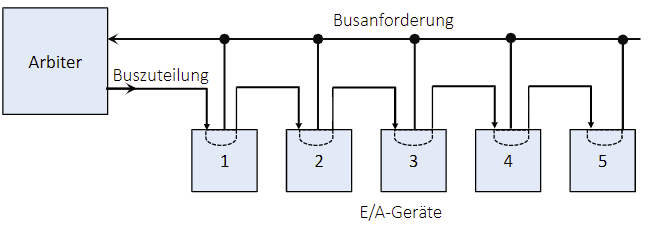
\includegraphics[scale=0.6]{15.png}
\end{center}

$\rightarrow$\textbf{Daisy Chain} 

Je näher ein Gerät am Arbiter liegt, desto höher seine Priorität. Um diese zu umgehen können z.B.mehrere Prioritätsebenen eingesetzt werden.

设备离仲裁器越近,其优先级越高。 为了避免这种情况,例如可以使用几个优先级。

\subsubsection{Dezentrale Busarbitrierung}

Gerät möchte senden (Busmaster werden):

Arbitrationsignal 仲裁信号:

\indent\indent 1 = Busmasterport frei $\rightarrow$ 0 senden und BUSY und Busmaster werden

\indent\indent 0 oder BUSY = Jemand ist bereits Busmaster $\rightarrow$ Signal durchgeben

Gerät mit IN aktiv wird Busmaster, Aktiviert BUSY und startet Sendevorgang.

Wer nicht senden will, reicht das aktuelle Signal durch.

\begin{center}
    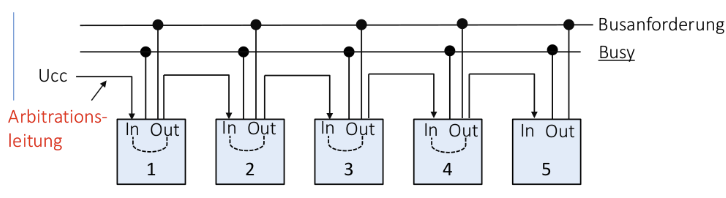
\includegraphics[scale=0.5]{16.png}
\end{center}

\section{Memory-Mapped IO (Vollständig / partiell)}

\noindent Verschiedene Geräte müssen über den Adressbus angesprochen werden können.

\noindent 必须能够通过地址总线对各种设备进行寻址。


\subsection{Vorgehensweise vollständiges Mapping: 完整的映射过程} 

Bei vollständigem Memory-Mapping werden die Geräte (ein)eindeutig auf dem Bus angeschlossen.

通过完整的内存映射,设备(打开)可以清楚地连接到总线。
\\
\\
\indent 1) Anzahl der möglichen Adressen und Anzahl der Leitungen. Z.B. 16-Bit Adressbus $\rightarrow$ 16 Leitungen (0....15) und $2^{16}$ = ca. 64K Adressen verfügbar.

可能的地址数和行数。 例如16位地址总线$ \rightarrow $ 16行(0 .... 15)和$ 2 ^ {16} $ =大约有64K地址可用。

若给了条件Speicherchips von jeweils 16kB, 那么可以算有多少个Speicherchips与处理器相连接:

64KB/16KB = 4 Speicherchips
\\
\\
\indent 2) Anzahl der Leitungen bestimmen, die für die einzelnen Geräte zur Adressierung genutzt werden können. Z.B. 2-KB-XXX $\rightarrow$ $2^{11}$ interne Adressen, d.h 16-11 = 5 Leitungen zur Adressierung müssen genutzt werden.

确定可用于单个设备寻址的线数。 例如2-KB-XXX$\rightarrow 2 ^ {11} $内部地址,即16-11 = 5行用于寻址。

z.B. 3-Port-PIO $\rightarrow 2^3$ nötig um alle ,,interne Adressen'' abzubilden, d.h 16-3=13 Leitungen zur Adressierung müssen genutzt werden.

例如,映射所有“内部地址”所需的3端口PIO$\rightarrow 2 ^ 3 $,即必须使用16-3 = 13行。
\\
\\
\indent 3) Geräte auf dem Adressbereich zuordnen, unter Beachtung ihrer Größe. (2KB-Gerät braucht 2048 freie Adressen danach). Beispiel mit 2-KB-EPROM, 2-KB-RAM und 3-Port-PIO:

考虑到设备的大小,将设备分配到地址范围。 (之后2KB的设备需要2048个空闲地址)。 2 KB EPROM,2 KB RAM和3端口PIO的示例:

\begin{center}
    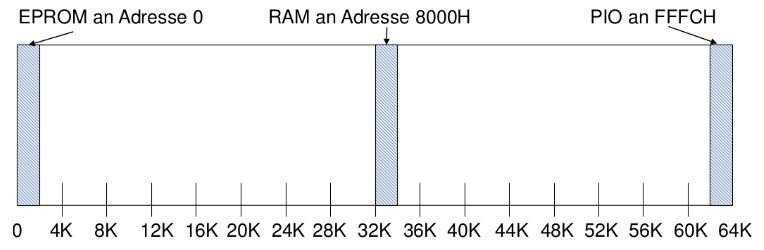
\includegraphics[scale=0.5]{17.png}
\end{center}

4) Bitfolge der Anordnungen finden:

\indent\indent Hier: EPROM: 0000 0-{}-{}- -{}-{}-{}- -{}-{}-{}-

\indent\indent\indent RAM:  1000 0-{}-{}- -{}-{}-{}- -{}-{}-{}-

\indent\indent\indent PIO:  11111 1111 1111 1-{}-{}-

Hinweis: Die Bitfolge ergibt sich einfach aus der Position der Geräte im Adressbereich, dabei teilt jedes Bit den Bereich in eine Hälfte, also das erste Bit in 32K, das zweite in 16K, das dritte in 8K, usw.

注意:位序列是由设备在地址区域中的位置产生的,每个位将区域划分为一半,即第一位为32K,第二位为16K,第三位为8K,依此类推。

Also z.B. 01011 würde bei Adresse 22K beginnen (0 – zwischen 0 und 32, 1 zwischen 16 und 32, 0 zwischen 16 und 24, 1 zwischen 20 und 24, 1 zwischen 22 und 24)

因此,例如01011将从地址22K开始(0-在0和32之间,1在16和32之间,0在16和24之间,1在20和24之间,1在22和24之间)
\\
\\
5) Anordnung zeichnen.

Vorgehensweise bei partieller Adresscodierung 部分地址编码的过程:

Die Vorgehensweise ist ähnlich wie bei der vollständigen Codierung, mit dem Unterschied, dass nurdie minimal benötigte Anzahl an Leitungen genutzt wird, um ein bestimmtes Gerät eindeutig zu identifizieren.

该过程类似于完整编码的过程,不同之处在于,仅使用最少数量的行来唯一地标识特定设备。

Nach obigem Beispiel ergibt sich 根据上面的示例:

- EPROM: 0 $\rightarrow$ a alle Leitungen auf 0 sein müssen um das Teil anzusprechen, brauchen min. also nur eine 0.

- 所有行必须在0上才能寻址该部件,因此它们仅需要0

- RAM: 10 $\rightarrow$ da bei 32K anliegt, und nur das erste Bit deshalb 1 sein muss.

- 因为存在32K,因此仅第一位必须为1。

- PIO: 11 $\rightarrow$ da die obersten Stellen alle 1 sind. 因为前两位都是1。
\\
\\
\indent$\rightarrow$ Brauchen bei RAM und PIO je zwei Stellen, da sie alle oberhalb von 32K liegen, würde z.B. RAM die 0 fehlen, wäre die Zuordnung nicht mehr ganz klar.

$\rightarrow$ 如果RAM和PIO都需要两位数字,因为它们都在32K以上,例如,如果RAM缺少0,则分配将不再十分清楚。

\section{Zahlenumwandlung}

\noindent\underline{10 $\rightarrow$ 2}

\noindent\textit{Bsp. $13_{10}$}

13 : 2 = 6 R 1

6 : 2 = 3 R 0

3 : 2 = 1 R 1

1 : 2 = 0 R 1

$\rightarrow$ $1101_2$
\\
\\
\noindent\textit{Bsp. $34.3125_{10}$}

34 = $2^5+2^2$ = 100010

2 $\times$ 0.3125 = 0.625 $<$ 1 $\Rightarrow$ 0

2 $\times$ 0.625 = 1.25 $\geq$ 1 $\Rightarrow$ 1

2 $\times$ 0.25 = 0.5 $<$ 1 $\Rightarrow$ 0

2 $\times$ 0.5 = 1 $\geq$ 1 $\Rightarrow$ 1

$\rightarrow$ $100010.0101$
\\
\\
\noindent\underline{2 $\rightarrow$ 10}

\noindent\textit{Bsp. $101.00101_{2}$}

$101.00101_2 = 2^2 + 2^0 + 2^{-3} + 2^{-5}=4+1+\frac{1}{8} + \frac{1}{32}=5.15625_{10}$
\\
\\
\noindent\underline{16 $\rightarrow$ 10}

\noindent\textit{Bsp. $2B_{16}$}

$2B_{16} = 2\times 16^1 + B\times 16^0 = 32 + 11 = 43_{10}$
\\
\\
\noindent\underline{10 $\rightarrow$ 16}

\noindent\textit{Bsp. $796_{10}$}

796 : 16 = 49 R 12 $\Rightarrow$ C

49 : 16 = 3 R 1

3 : 16 = 0 R 3

$\rightarrow$ 31C
\\
\\
\noindent\underline{2 $\rightarrow$ 16}

\noindent\textit{Bsp. $1101 0111_{2}$}

0111 = 7

1101 = D

$\rightarrow$ D7
\\
\\
\noindent\underline{16 $\rightarrow$ 2}

\noindent\textit{Bsp. $D7_{16}$}

D = 1101

7 = 0111

$\rightarrow$ 1101 0111

\section{Floating Points}

\begin{center}
    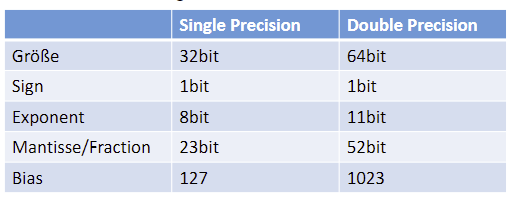
\includegraphics[scale=0.6]{18.png}
\end{center}

\subsection{Bias 偏差:} 

Bias wandelt einen signed Exponenten (127 bis +127) in einen unsigned value um $\rightarrow$ Wird addiert zum eigentlichen Exponenten.

偏差将带符号的指数(127到+127)转换为无符号值$\rightarrow$加到实际的指数上。

\subsection{Sonderfälle in der IEEE 754 Norm}

\begin{center}
    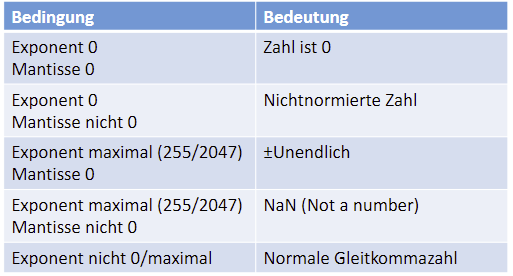
\includegraphics[scale=0.6]{19.png}
\end{center}

Negative Exponenten einer Gleitkommazahl werden nach der Norm IEEE 754 als Zweierkomplementzahl dargestellt. (Falsch)

根据IEEE 754标准,浮点数的负指数表示为二进制补码。(错)

\section{Rechnen in Normdarstellung}

\noindent\textit{3.9 $\rightarrow$ Single- und Double-Precision}

$3.9_{10}=11.1\quad 1100\quad 1100\quad 1100\quad 1100 \dots \times 2^0$

$3.9_{10} = 1.11\quad 1100\quad 1100\quad 1100\quad 1100\dots\times 2^1$

\begin{center}
    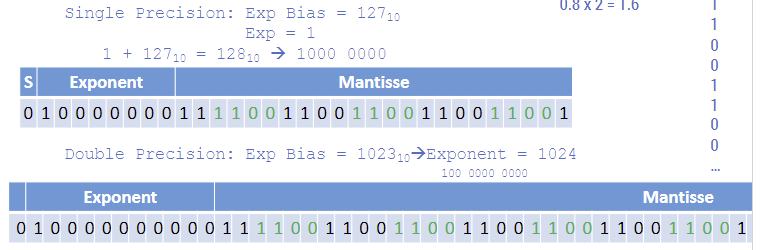
\includegraphics[scale=0.5]{20.png}
\end{center}

\noindent\textit{Single-Precision $\rightarrow$ Dezimalzahl}

\begin{center}
    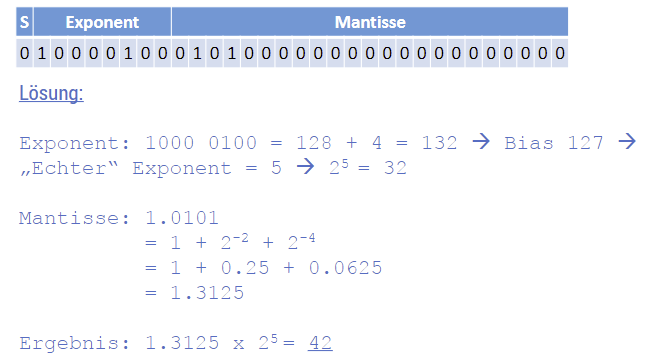
\includegraphics[scale=0.5]{21.png}
\end{center}

\noindent\underline{Addition:}

1) Exponenten angleichen (den der kleineren Zahl nach rechts schieben)

2) Mantissen addieren

3) Normdarstellung (prüfen)

4) evtl. Abrundung und zurück zu 3)

\noindent\underline{Multiplikation:}

1) Berechnung des Exponenten vom Produkt ( E1 +  E2 – Bias)

2) Multiplikation der Mantissen

3) + 4) siehe Addition

5) Vorzeichen berechnen (VZ unterschiedlich → negativ, ansonsten positiv)

\noindent\underline{加法:}

1)调整指数(将较小的数字向右移动)

2)添加尾数

3)标准表示(检查)

4)可能会四舍五入并返回到3)

\noindent\underline{乘法:}

1)计算乘积的指数(E1 + E2-偏差)

2)尾数相乘

3)+ 4)见加法

5)计算符号(VZ不同→负,否则为正)
\\
\\
\noindent\textit{Bsp.}

\textit{Führen sie die Gleitkomma-Addition/Multiplikation der folgenden Zahlen durch, wenn 4 Bit Mantisse und 2 Bit Exponent verwendet werden: a)$2.25_{10}$, b)$-0.75_{10}$}

\textit{\textbf{Addition:}}

1)

\indent\indent$2.25_{10}=1.001_2\times 2^1$

\indent\indent$-0.75_{10}=-1.1_2\times 2^{-1}$

2)

\begin{center}
    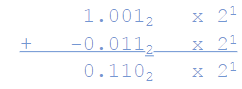
\includegraphics[scale=0.5]{22.png}
\end{center}

3) $1.1000\times 2^0$

4) Nicht notwendig $\rightarrow$ $1.1000\times 2^0$
\\
\\
\indent\textit{\textbf{Multiplikation:}}

\begin{center}
    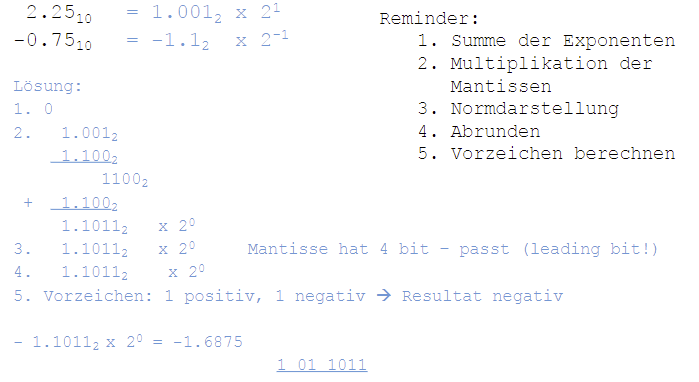
\includegraphics[scale=0.5]{23.png}
\end{center}

\section{MIPS-Assemblersprache}

\subsection{weriteren Operationstypen:}

\begin{center}
    \begin{tabular}{|l|l|}
        \hline
        Type&Beispiel\\
        \hline
        Logische&And, Or, Nor, Shift\\
        \hline
        Transfer&Load, Store\\
        \hline
        Bedingte Verzweigungen&Branch on X, set on X\\
        \hline
        Unbedingter Sprung&jump\\
        \hline
    \end{tabular}
\end{center}

\subsection{Wieviele Register hat MIPS und welche Nomenklatur haben diese?}

32 - Format:\$12

\begin{center}
    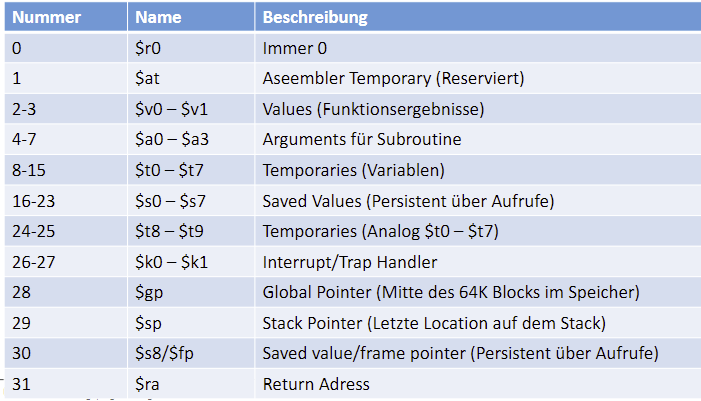
\includegraphics[scale=0.5]{24.png}
\end{center}

\subsection{möglichen Fragen}

\noindent\underline{\textbf{NOT} Operation: a = NOT b}

Nor-Opration mit 0, a, b gespeichert in \$s0, \$s1.

$\rightarrow$ z. B.\qquad b = 00 1100 1010, a = NOT b

\indent\indent läß\qquad  \$t0 = 00 0000 0000

\indent\indent gilt: \quad a = b NOR \$t0

\indent\indent $\Rightarrow$ nor \$s0, \$s1, \$t0
\\
\\
\noindent\underline{Der Befehl ,,add'' ist der langsamste in MIPS.} (Falsch) 加法最慢(错)
\\
\\
\noindent\underline{Im Gegensatz zu einem Single-Cycle-Datenpfad können Befehle bei einem Multi-Cycle-}

\underline{Datenpfad nicht länger als 3 Taktzyklen sein.}(Falsch)

与单周期数据路径相比,多周期数据路径中的命令不能超过3个时钟周期。(False)
\\
\\
\noindent\underline{Befehlstype in MIPS}

\begin{center}
    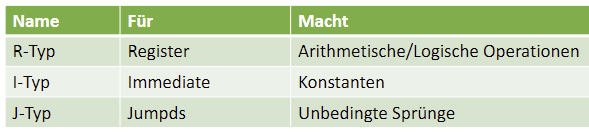
\includegraphics[scale=0.5]{25.png}
\end{center}

\subsection{R-Typ-Befehls}

\begin{center}
    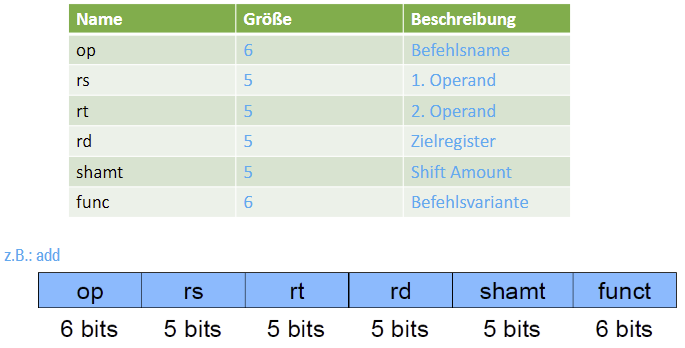
\includegraphics[scale=0.5]{26.png}
\end{center}

R-Typ-Befehle besitzen ein zusätzliches Feld für den „Function Code“, da gewisse R-Typ-Befehle den gleichen OPCode haben.(Richtig)

由于某些R型命令具有相同的OP代码,因此R型命令具有“功能代码”的附加字段。(对)

\subsection{I-Typ-Befehls}

\begin{center}
    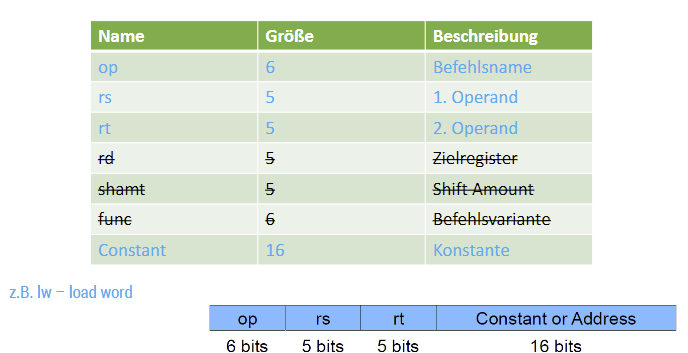
\includegraphics[scale=0.5]{27.png}
\end{center}

\subsection{J-Typ-Befehls}

\begin{center}
    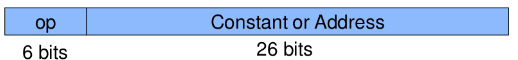
\includegraphics[scale=0.5]{28.png}
\end{center}

\section{MIPS-Speicher}

- Big-Endian

- 32-Bit-Words werden in 4-Byte-Bereiche aufgeteilt

\begin{center}
    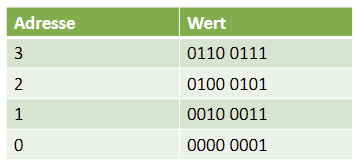
\includegraphics[scale=0.5]{29.png}
\end{center}

- Word–Aligned (jeder Word endet sich mit 00) (d.h Adresse +1 ist z.B. Adresse 80 $\rightarrow$ nächste Adresse 84)

- Achtung! Multiplikation (mit 4) der Adressen geschieht Hardwareseitig, d.h. Will ich auf 10.000 springen muss ich nur 2.500 angeben, d.h. will ich auf Arraystelle 3 (an Adresse 12) zugreifen, reicht es 3 zu schreiben.

- 注意!地址的乘数(乘以4)是在硬件方面完成的,即,如果我想跳到10000,我只需要指定2500,即,如果我要访问数组位置3(在地址12),写3就足以。

\subsection{möglichen Fragen}

\noindent\underline{In MIPS wird beim Instruction Fetch (Befehl laden) der Program Counter um 4 inkrementiert.} 

(Richtig)

\underline{在MIPS中,在指令获取(装入命令)期间,程序计数器增加4。} (对)
\\
\\
\underline{Program-Counter-relative Adressierung ist in MIPS nicht möglich.}(Falsch)

\underline{在MIPS中无法实现程序计数器相对寻址。}(错)
\\
\\
\noindent\underline{Mashinencode $\leftrightarrow$ C-Programm?}

\noindent\textbf{a)} A[125] = h - A[25];  \qquad\qquad//\$t1 : A, \$s0 : h

\indent\indent lw \$t0, 25(\$t1)

\indent\indent sub \$t0, \$s0, \$t0

\indent\indent sw \$t0, 125(\$s1)
\\
\\
\textbf{b)}

\begin{lstlisting}
i = 0 ; 
while (A[i] != 10 && i < 10) 
    A[i] = i ; 
    i = i + 1 ;
end while
\end{lstlisting}

\begin{lstlisting}
        and $s2, $s2, $zero         # i = 0 
        addi $s3, $zero, 10         # $s3 = 10
Loop:   sll $t1, $s2, 2             # mal 4, weil Wörter
        add $t1, $t1, $s1           # $t1 = Adresse 
        lw $s4, 0($t1)              # Laden von A[i]
        beq $s4, $s3, Exit          # A[i] = 10 -> Exit 
        sw $s2, 0($t1)              # A[i] = i 
        addi $s2, $s2, 1            # i = i + 1
        beq $s2, $s3, Exit          # i = 10 -> Exit 
        j Loop                      # A[i] != 10 && i < 10 -> Loop
Exit: 
\end{lstlisting}

\noindent\textbf{c)}

\begin{lstlisting}
int * multi(int scalar, int vector_x, int vector_y){
    int s = scalar;     

    //v_x 所有元素用"vector_x" 初始化
    int v_x[100] = {vector_x};

    //v_y 所有元素用"vector_y" 初始化
    int v_y[100] = {vector_y};

    int result[100];

    for(int i = 0; i < 100; i++){
        result[i] = s * v_x[i] + v_y[i];
    }

    return result;
}    
\end{lstlisting}

\begin{lstlisting}
lw $t2, 0($t7)              ;load scalar s
add $t3, $t0, 400           ;save max_index100 to register $t3
loop:   lw $t4, 0($t0)      ; load x[i]
        lw $t5, 0($t1)      ; load y[i]
        mult $t2, $t4       ; save s*x[i] to register $LO
        add $t6, $LO, $t1   ; save $LO+y[i] to register $t6
        sw $t6, 0($t8)      ; save result[i]
        addiu $t0, $t0,4    ;i++
        addiu $t1, $t1,4
        addiu $t8, $t8,4
        bne $t0, $t3, loop  ;continue loop when i!=100
\end{lstlisting}






\section{Datenpfade und Pipelines 数据路径和管道}

\noindent Ein MIPS-Befehl besteht aus 5 Phasen:

\begin{center}
    \begin{tabular}{|c|c|c|c|c|c|}
        \hline
        &1&2&3&4&5\\
        \hline
        Load&IF&ID/RF&ALU/EX&Mem&WB\\
        \hline
    \end{tabular}
\end{center}

IF - InstructionFetch

ID/RF - InstructionDecode/Register Fetch

ALU/EX - Executiondurch ALU

Mem - Memory Access

WB - Writeback

\subsection{möglichen Fragen}

\noindent\underline{Eine Pipeline ermöglicht, Teile der Rechnerbefehle sequentiell zu einander auszuführen.} (Falsch)

流水线使部分计算机指令可以彼此顺序执行。(错)
\\
\\
\noindent\underline{Welche Einschränkungen existieren für die Parallelität durch Pipelines?}

\underline{通过管道进行并行性有哪些限制?}

Es dürfen keine Abhängigkeitenbestehen. 必须没有依赖关系。

\begin{center}
    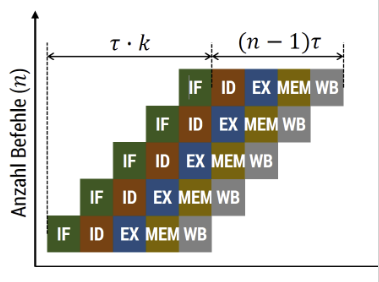
\includegraphics[scale=0.5]{30.png}
\end{center}

\subsection{Datenabhängigkeiten 数据依存关系}

-Namensabhängigkeiten (auch unechte Datenabhängigkeiten) 名称依赖性(也包括虚假数据依赖性)

-Kontrollflussabhängigkeiten 控制流依赖性

-echte Datenabhängigkeiten 实际数据依赖
\\
\\
Wie sind die Datenabhängigkeiten charakterisiert? 数据依赖关系如何表征?

\begin{center}
    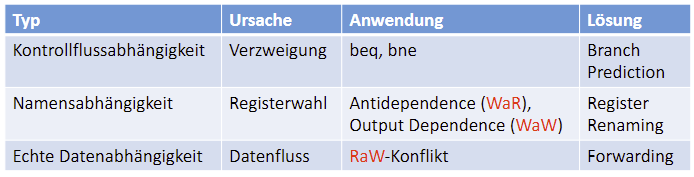
\includegraphics[scale=0.5]{31.png}
\end{center}

$\rightarrow$ 3 große \textbf{Datenkonflikte (Data Hazards)} 3大数据冲突(数据危害)

WaR-Write after Read    \qquad\qquad     -b schreibt Wert bevor a den ,,alten'' lesen kann

b在a可以读取“旧”值之前写值

WaW-Write after Write     \qquad\qquad  -a und b schreiben in falscher Reihenfolge

a和b以错误的顺序书写

RaW-Read after Write       \qquad\qquad  -a liest Wert bevor er von b fertig geschrieben ist

a在b完成之前读取值
\\
\\
Welche \textbf{Konsequenz haben Data Hazards} auf die Pipeline-Ausführung? 数据危害对管道执行有何影响?

Wartezyklen (Stalls) um Hazards zu vermeiden $\rightarrow$ Reduziert Effizienz der Pipeline.

等待周期(排程)以避免危险->降低管道效率。

\begin{center}
    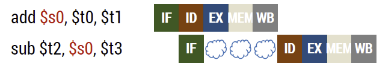
\includegraphics[scale=0.5]{32.png}
\end{center}

Lösungen: Umsortieren, Forwarding, Register Renaming, Branch Prediction
\\
\\
\noindent\underline{Bsp. Data Hazards 数据危害}

\begin{center}
    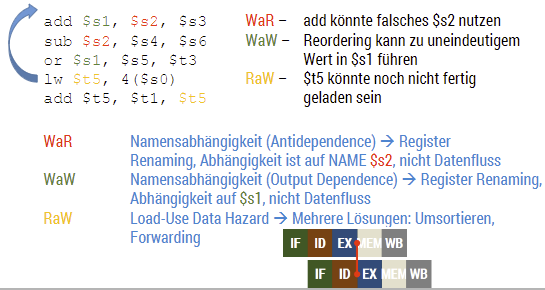
\includegraphics[scale=0.6]{33.png}
\end{center}

WaR: Namensabhängigkeit (Antidependence) $\rightarrow$ Register Renaming, Abhängigkeit ist auf NAME \$s2, nicht Datenfluss.

WaR:名称依赖性(Antidependence)$ \rightarrow $寄存器重命名,依赖性取决于NAME \$s2,而不是数据流。

WaW: Namensabhängigkeit (Output Dependence) $\rightarrow$ Register Renaming, Abhängigkeit auf \$s1, nicht Datenfluss

WaW:名称依赖(输出依赖)$ \rightarrow $寄存器重命名,依赖\$s1,而不是数据流

RaW: Load-Use Data Hazard $\rightarrow$ Mehrere Lösungen: Umsortieren, Forwarding.

RaW:负载使用数据危害$ \rightarrow $几种解决方案:重新排序,转发。
\\
\\
\noindent\underline{Bsp. Problematik}

add \$t1, \$t2, \$t3

bne \$s2, \$s3, label

sub \$s1, \$s6, \$s4 \qquad\qquad $\leftarrow$ Notwendig?

\textbf{Ans:} Sprungergebnisse erst im Write-Back bekannt $\rightarrow$ Delayed alles

仅在回写中知道跳转结果 $\rightarrow$ 延迟一切

$\rightarrow$ Stalling - Einfach, aber ineffizient 停转-简单但效率低下

$\rightarrow$ Delayed Branch - Nächste Instruktion präventiv auch ausführen 延迟分支-也预防性地执行下一条指令

$\rightarrow$ Sprungvorhersage - Statisch und dynamisch 跳跃预测-静态和动态

\subsection{statische und dynamische Sprungvorhersage 静态和动态跳转预测}

\textit{Wodurch unterscheiden sich \underline{statische und dynamische Sprungvorhersage}?}

\noindent\textit{\underline{静态和动态跳转预测}有何区别?}

\begin{center}
    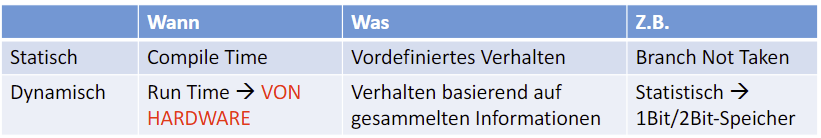
\includegraphics[scale=0.5]{34.png}

    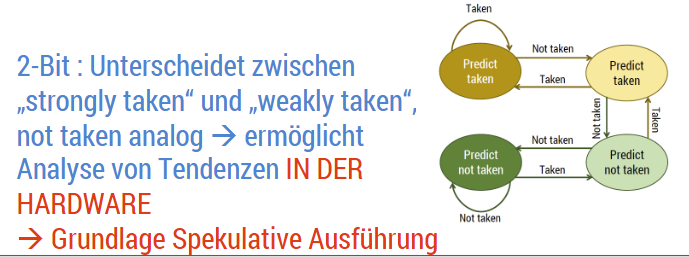
\includegraphics[scale=0.6]{35.png}
\end{center}

\noindent 2-Bit: 区分“强采纳”和“弱采纳”,而不是模拟采纳。$\rightarrow$ 能够分析\textbf{硬件}趋势$\rightarrow$基于投机执行
\\
\\
\underline{zwei Branch-Prediction-Strategien} 两种分支预测策略

Statisch, Dynamisch 

Always Taken, Never Taken 

Forward never backward always
\\
\\
\noindent\underline{Unterschied zwischen einer \textbf{Abhängigkeiten (Dependence)} und einem \textbf{Konflikten (Hazard)}}

$\circ$ Datenabhängigkeit (Dependency) - Eigenschaft eines Programmes

$\circ$ 数据依赖关系(Dependency)-程序的属性

$\circ$Hazard - Potentielles Problem aus einer Abhängigkeit, hängt jedoch von der Hardware ab! Programand ProcessorOrganisation

$\circ$ 危险-潜在的依赖关系问题,但取决于硬件! 程序和处理器组织

$\rightarrow$ Nicht jede Abhängigkeit führt zu einem Konflikt - Hängt von der Pipeline ab

$\rightarrow$ 并非每个依赖项都会导致冲突-取决于管道

\newpage

\begin{center}
    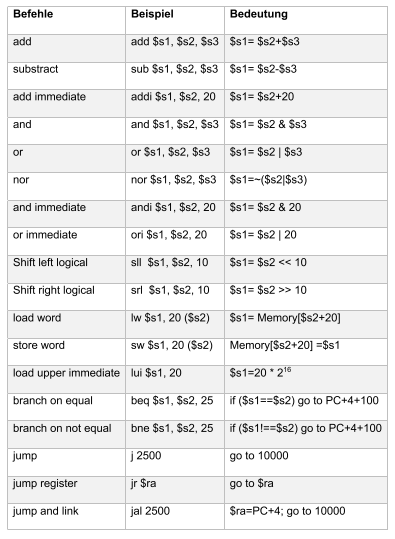
\includegraphics[scale=1]{36.png}
\end{center}



















\end{document}